\documentclass[conference]{IEEEtran}

\usepackage[T1]{fontenc}
\usepackage{cite}
\usepackage{amsmath,amssymb}
\usepackage{booktabs}
\usepackage{array}
\usepackage{xcolor}
\usepackage{listings}
\usepackage{pgfplots}
\pgfplotsset{compat=1.16}
\usepackage[colorlinks=true,linkcolor=black,citecolor=black,urlcolor=black,
            pdftitle={Training a Masked Diffusion Language Model on a Single Laptop},
            pdfauthor={Aditya Dutt Pandey}]{hyperref}

\lstset{basicstyle=\ttfamily\scriptsize, breaklines=true, frame=single,
        columns=fullflexible, keepspaces=true}

\newcommand{\mask}{\texttt{[MASK]}}
\newcommand{\xzero}{\mathbf{x}_0}
\newcommand{\xt}{\mathbf{x}_t}

\begin{document}

\title{Training a Masked Diffusion Language Model\\on a Single Laptop}

\author{\IEEEauthorblockN{Aditya Dutt Pandey}
\IEEEauthorblockA{GitHub: Adityaadpandey\\
\url{https://github.com/Adityaadpandey/diffusion\_llm}}}

\maketitle

\begin{abstract}
This paper describes a small masked diffusion language model that was
implemented from scratch and trained on the TinyStories corpus using one
Apple M4 Pro laptop. The model starts from a fully masked sequence and fills it
in over a few dozen denoising passes instead of decoding left to right. The
reference model has 41.2M parameters and trains in 3 h 41 min. It reproduces the
style of the corpus, including character names, short sentences and quoted
dialogue, but it does not sustain a plot beyond a sentence or two. Two of three
full runs failed to learn beyond unigram statistics. The third trained normally
after the loss and the diffusion horizon were changed together; because the
ablation separating the two changes was not run, the cause is reported as a
hypothesis. The paper also documents a validation metric that overstates model
quality and three defects found in the implementation.
\end{abstract}

\begin{IEEEkeywords}
masked diffusion, discrete diffusion, language modeling, TinyStories,
parallel decoding, small-scale training
\end{IEEEkeywords}

\section{Introduction}

Autoregressive transformers generate text in one direction: token $n$ is chosen
given tokens $1,\dots,n-1$. The approach is simple and works well, but it
imposes three constraints. Producing $L$ tokens takes $L$ sequential forward
passes, a token cannot be revised once written, and conditioning on text that
lies to the right of a position requires additional training or prompting
tricks.

Masked diffusion language models remove the left-to-right order
\cite{austin2021d3pm,sahoo2024mdlm,lou2024sedd}. A bidirectional transformer is
trained on text in which a random subset of tokens has been replaced by a
\mask{} symbol, at every corruption level from nearly clean to fully masked.
Generation starts from all \mask{} and applies the model repeatedly, committing
some tokens at each pass. At the 8B scale this approach has been reported to be
competitive with autoregressive models of similar size \cite{nie2025llada}.

This work asks how much of that behaviour survives at a very small scale, on one
consumer machine and without cloud compute. No new method is proposed. The
contributions are:
\begin{itemize}
\item a compact PyTorch implementation of masked diffusion for text with two
      denoiser architectures and two samplers;
\item a 41.2M-parameter model trained on TinyStories in under four hours,
      with its validation curve and samples;
\item a record of two failed runs and of the change that fixed training; and
\item an account of the weaknesses of the evaluation metric and of three
      implementation defects.
\end{itemize}

\section{Related Work}

D3PM \cite{austin2021d3pm} extended diffusion to discrete data and introduced
corruption into an absorbing \mask{} state. SEDD \cite{lou2024sedd} trains by
estimating ratios of the data distribution. MDLM \cite{sahoo2024mdlm} showed
that a simple masked objective with a good training recipe is competitive among
diffusion language models, and LLaDA \cite{nie2025llada} scaled it to 8B
parameters. Diffusion-LM \cite{li2022diffusionlm} instead diffuses in a
continuous embedding space.

Committing the most confident predictions first and leaving the rest masked
comes from MaskGIT \cite{chang2022maskgit} for images and Mask-Predict
\cite{ghazvininejad2019maskpredict} for translation. The denoiser is an
encoder-only transformer \cite{vaswani2017attention,devlin2019bert}. One of the
two implemented variants conditions on the timestep with adaLN-Zero
\cite{peebles2023dit} and uses rotary position embeddings
\cite{su2021roformer}. The data is TinyStories \cite{eldan2023tinystories}, a
synthetic corpus of short stories with a toddler-level vocabulary. None of these
ideas originate here. The implementation, training configurations, experimental
record and analysis are the work of this paper.

\section{Method}

\subsection{Forward Corruption Process}

Let $\xzero$ be a sequence of $L$ token ids and $t\in\{1,\dots,T\}$ a timestep.
A schedule maps $t$ to a masking probability $\beta(t)$, and each token is
independently replaced by \mask{} with that probability. The reference run uses
the cosine schedule with $T=100$:
\begin{equation}
  \beta(t)=1-\cos\!\Big(\frac{t}{T}\cdot\frac{\pi}{2}\Big).
\end{equation}
Linear and square-root schedules are also implemented. With $t$ uniform, the
mean masking rate is $1-2/\pi\approx0.363$, which matters for the metric
discussed in Section~\ref{sec:metric}.

\subsection{Denoiser}

The model $p_\theta(\xzero\mid\xt,t)$ outputs a distribution over the
vocabulary at every position. Attention is bidirectional (no causal mask) and
the output projection is tied to the token embedding. The repository contains
two architectures, distinguished at load time from the tensor names in the
checkpoint.

The \emph{legacy} architecture produced all reported results. Its input is the
sum of a token embedding, a learned position embedding and a projected
sinusoidal timestep embedding, followed by $N$ pre-LayerNorm encoder blocks and
a final LayerNorm. The noise level is injected once, so the network must carry
it through its depth.

The second architecture, implemented but not yet trained, follows DiT
\cite{peebles2023dit}. A small MLP maps the timestep to a conditioning vector
$c$, and each block derives a shift $b$, scale $s$ and gate $g$ for each of its
two sublayers:
\begin{equation}
  \mathbf{h}\leftarrow\mathbf{h}+g\odot
  \mathrm{Sublayer}\big(\mathrm{LN}(\mathbf{h})\odot(1+s)+b\big).
\end{equation}
The layers producing $b$, $s$, $g$ are zero-initialised so every block starts
as the identity. Rotary embeddings replace the learned position table.

\subsection{Training Objective}

For each sequence, $t$ is drawn uniformly, $\xzero$ is corrupted to $\xt$, and
the cross-entropy to $\xzero$ is averaged over \emph{all} positions, masked or
visible:
\begin{equation}
  \mathcal{L}(\theta)=\mathbb{E}\Big[\frac1L\sum_{i=1}^{L}
  -\log p_\theta\big(x_0^{(i)}\mid\xt,t\big)\Big].
\end{equation}
This differs from the weighted masked-position ELBO of MDLM, because the model
is also trained to copy visible tokens. Section~\ref{sec:failures} suggests
this choice is important.

\subsection{Sampling}

Generation starts from $L$ masked positions, optionally with fixed prompt
tokens, and runs $N$ steps. At each step the model predicts every position and
a sampler decides which masked positions to commit.

The \emph{posterior} sampler is the exact reverse of the corruption. A position
masked at time $t$ was still masked at an earlier time $t'$ with probability
$\beta(t')/\beta(t)$. Each masked position therefore stays masked with that
probability and is otherwise drawn from the model; filled positions never
change. This sampler is used for all reported samples (32 steps, temperature
1.0, top-$k$ 40).

The \emph{confidence} sampler follows MaskGIT. It ranks masked positions by the
model's top probability and commits the highest-ranked ones, using a sampled
token because the argmax would make all samples identical. The number of
positions still masked after step $k$ of $N$ is
$\mathrm{round}\big(n_0\cos(\tfrac{\pi}{2}\tfrac{k+1}{N})\big)$, which
guarantees a complete sequence after the last step.

\subsection{Data}

Stories are tokenized, joined with a separator and cut into fixed chunks of 128
tokens; 0.5\% is held out for validation. The reference run uses
\texttt{bert-base-uncased}, so all text is lowercase. GPT-2 style BPE
tokenizers are supported by the code but were not used for training.

\section{Experimental Setup}

All values come from the configuration files and training logs in the
repository (Table~\ref{tab:setup}).

\begin{table}[t]
\centering
\caption{Reference run (\texttt{tinystories\_fast.yaml}).}
\label{tab:setup}
\footnotesize
\begin{tabular}{@{}l>{\raggedright\arraybackslash}p{0.68\columnwidth}@{}}
\toprule
Hardware & Apple M4 Pro, 24 GB, PyTorch MPS, bf16 autocast \\
Parameters & 41,175,552 ($d{=}512$, 8 layers, 8 heads, $d_\text{ff}{=}2048$) \\
Architecture & Legacy: learned positions, timestep added at input \\
Tokenizer & \texttt{bert-base-uncased}, vocabulary 30,522 \\
Data & TinyStories train, 2,119,719 stories, $\approx$2.09M chunks (268M tokens) \\
Diffusion & $T{=}100$, cosine schedule, loss on all positions \\
Optimizer & AdamW \cite{loshchilov2019adamw}, lr $3{\times}10^{-4}$, $\beta{=}(0.9,0.98)$, weight decay 0.01, clip 1.0 \\
Batch & $24\times6$ accumulation = 144 sequences ($\approx$18k tokens) \\
Length & 50,000 micro-batches, 8,333 updates, 154M tokens ($\approx$0.57 epoch) \\
Time & 3 h 41 min ($\approx$3.8 micro-batches/s) \\
Sampling & 32 steps, posterior, temperature 1.0, top-$k$ 40 \\
Seed & 42, single run \\
\bottomrule
\end{tabular}
\end{table}

\section{Results}

Fig.~\ref{fig:val} shows the validation score, logged every 2,500
micro-batches, for the reference run and the two earlier failed runs. Each
evaluation draws one random $t$ per validation sequence, so points are noisy.
The reference score falls from 9.2 at step 7,500 to 3.79 at step 45,000, and the
final training loss is about 1.13 nats per position.

\begin{figure}[t]
\centering
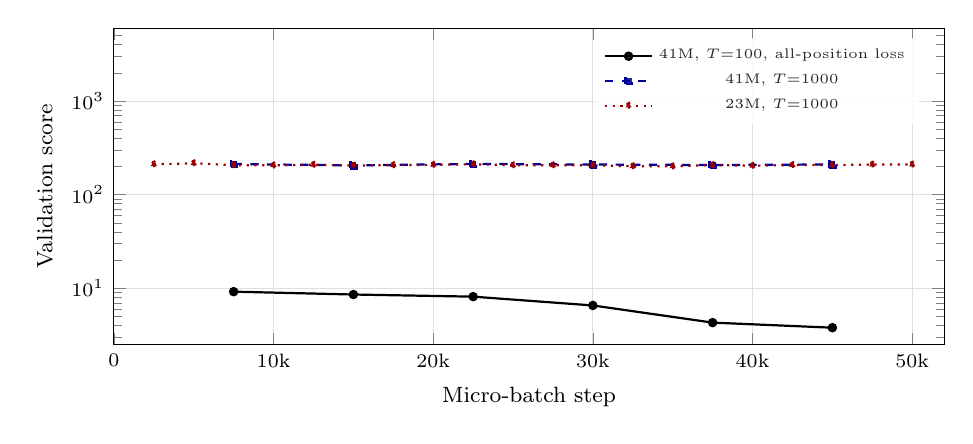
\begin{tikzpicture}
\begin{axis}[
  width=\columnwidth, height=5.6cm,
  xlabel={Micro-batch step}, ylabel={Validation score},
  ymode=log, ymin=2.5, ymax=6000,
  xmin=0, xmax=52000,
  xtick={0,10000,20000,30000,40000,50000},
  xticklabels={0,10k,20k,30k,40k,50k}, scaled x ticks=false,
  grid=major, grid style={gray!25},
  legend pos=north east,
  legend style={font=\tiny, draw=none, fill=white, fill opacity=0.85},
  tick label style={font=\scriptsize}, label style={font=\footnotesize},
]
\addplot[color=black, mark=*, mark size=1.3pt, thick] coordinates {
  (7500,9.201) (15000,8.579) (22500,8.139) (30000,6.554) (37500,4.298) (45000,3.793)};
\addlegendentry{41M, $T{=}100$, all-position loss}
\addplot[color=blue!60!black, mark=square*, mark size=1.1pt, thick, dashed] coordinates {
  (7500,212.593) (15000,205.521) (22500,213.087) (30000,209.848) (37500,207.379) (45000,210.223)};
\addlegendentry{41M, $T{=}1000$}
\addplot[color=red!60!black, mark=triangle*, mark size=1.3pt, thick, dotted] coordinates {
  (2500,210.892) (5000,216.682) (7500,206.485) (10000,205.496) (12500,208.896) (15000,204.662)
  (17500,206.999) (20000,208.295) (22500,211.377) (25000,206.179) (27500,206.012) (30000,205.727)
  (32500,201.304) (35000,200.712) (37500,206.996) (40000,203.749) (42500,207.231) (45000,207.305)
  (47500,209.729) (50000,210.003)};
\addlegendentry{23M, $T{=}1000$}
\end{axis}
\end{tikzpicture}
\caption{Validation score of the three full runs (log scale). Both runs with
$T{=}1000$ remain near 200 for all 50,000 steps. The score is the exponential
of the all-position loss; see Section~\ref{sec:metric}.}
\label{fig:val}
\end{figure}

\subsection{Samples}

Unedited samples from the step-45,000 evaluation (first 200 characters,
32 steps, posterior sampler; lowercase is due to the tokenizer):
\begin{lstlisting}
. once upon a time there was a mouse. the
rat had very and he once upon a time there
was a mouse in his gray house. one day, it
found something on the ground. he ran
scared. the mouse decided to climb...

ben said, " but please want the bunny., i
do you you want to do. you can do? " the
bunny said. " i need you know. i know, i
want to help. i can ' t find me, " mia.
". but as they ran with the bunny. s...
\end{lstlisting}
The model reproduces the corpus register: names, short declarative sentences,
quoted dialogue and the conventional opening. It also shows the expected
failure modes of parallel decoding: repeated words (``you you''), contradictory
neighbouring clauses, and a story restarting midway. No automatic quality score
or human rating was computed, so this assessment rests on a small number of
outputs.

\subsection{Interpreting the Validation Score}
\label{sec:metric}

The score is not perplexity in the usual sense. It is the exponential of a loss
averaged over all positions, and on average only 36\% of positions are masked,
so about two thirds of the terms are near-zero copies. Since
$\ln 3.793\approx1.333$ nats per position, and masked positions can account for
at most all of it, the loss per masked token is bounded by
$1.333/0.363\approx3.67$ nats, a masked-token perplexity of at most about 39.
This bound was not measured directly. The score is meaningful only for
comparing runs of this same setup and must not be compared with perplexities
reported elsewhere.

\section{Analysis of the Failed Runs}
\label{sec:failures}

The first two runs, with 22.6M parameters ($d{=}384$, 6 layers) and 41.2M
parameters, both used $T{=}1000$. Each ran 50,000 steps and stayed at a score
of 200--217 with no downward trend. Their samples resembled
\texttt{to the to they said, a, a to was time play and and\dots}, which is
roughly what a model that knows only word frequencies produces.

The third run changed two things simultaneously: the loss moved from masked
positions to all positions, and $T$ was reduced from 1000 to 100. The score fell
from about 210 to 9.2 by step 7,500. A separate 1,000-step test of the
all-position loss reached 144, against about 203 for the earlier loss at the
same step count, which points to the loss as the main factor. A plausible
mechanism is that copying visible tokens provides an easy early signal that
stabilises training, but this was not tested. The controlled comparison
(all-position loss at $T{=}1000$, or masked-only loss at $T{=}100$) was not run,
so the attribution remains a hypothesis.

\section{Limitations}
\label{sec:limitations}

\subsubsection*{Coherence and parallel decoding}
The model is small, saw about half an epoch, and has no planning mechanism. With
32 steps over 128 tokens, roughly four tokens are committed per step without
seeing each other, which accounts for doubled words and clashing neighbours.
Quality as a function of step count was not measured.

\subsubsection*{Window and tokenizer}
The legacy model has exactly 128 learned positions and training chunks start and
end at arbitrary points, so generated stories begin and end mid-thought.
WordPiece lowercases text and decodes with stray spaces (``i can ' t''). A BPE
configuration exists but is untrained.

\subsubsection*{Implementation defects}
(i) \texttt{build\_model} in \texttt{src/train.py} does not pass
\texttt{use\_rope} or \texttt{rotary\_max\_seq\_len}, so a RoPE configuration
trains the learned-position model while saving a configuration that claims RoPE;
the reference run is unaffected. (ii) The training loop counts micro-batches
while the scheduler steps once per optimizer update, so the 2,000 warmup steps
last 12,000 micro-batches and cosine decay covers only about 13\% of its course
(final lr $2.89{\times}10^{-4}$ against a peak of $3{\times}10^{-4}$); it was
left unchanged so results remain reproducible. (iii) A docstring in
\texttt{diffusion\_loss} describes a weighted masked-position ELBO, whereas the
function computes the all-position mean.

\subsubsection*{Evaluation}
There are no downstream benchmarks, human ratings, repetition or diversity
scores, or autoregressive baseline of equal size and token budget, so no claim
is made about diffusion versus autoregressive generation. No speed advantage was
shown: every pass recomputes attention over the full sequence without caching,
and generation time was not compared with a baseline.

\subsubsection*{Reproducibility}
The checkpoint was produced by the legacy code at commit \texttt{0eab6d1}; later
commits changed the model and training script. A single seed was used and there
are no error bars.

\section{Future Work}

The next steps are to fix the two code defects; run the missing loss-versus-horizon
ablation; report a masked-token-only loss; train the adaLN and RoPE model with a
BPE tokenizer under identical seeds; measure quality against the number of
steps with repetition and distinct-$n$-gram scores; train an autoregressive
baseline of equal size and tokens; and evaluate remasking samplers and
unmasking orders that avoid committing conflicting neighbours. A 153M-parameter
configuration, requiring roughly a day on this hardware, should follow only
after these.

\section{Conclusion}

A masked diffusion language model can be trained from scratch on a laptop in
under four hours and generates text in the style of a children's story. Training
at this scale proved fragile: two of three runs learned nothing, and the reason
the third succeeded is only partly understood. The result is a baseline with its
flaws documented, from which the experiments above can be carried out.

\section*{Availability and License}

The code, configurations, logs and this paper are by Aditya Dutt Pandey and are
source-available under the license in the repository's \texttt{LICENSE} file;
all rights are reserved, and reuse, redistribution and presentation as another
person's work require written permission. The ideas cited here belong to their
original authors. The commit log records the history of the work.

\bibliographystyle{IEEEtran}
\bibliography{references}

\end{document}
